\documentclass[12pt]{article}

\usepackage{fontawesome}
\usepackage{hyperref}
\usepackage{xurl}
\usepackage{graphicx}

\hypersetup{
    colorlinks=false,
    pdfborder={0 0 0},
}


\title{Data Collection}
\author{
        Adrianna Holden-Gouveia \\
        Website: \url{https://aholdengouveia.name}\\ 
        \date{\vspace{-5ex}}
        %Email: \href{mailto:admin@aholdengouveia.name}{admin@aholdengouveia.name} \\
        \faLinkedin{: aholdengouveia} \\
        \faGithub {: aholdengouveia} \\
        %\faTwitter {: aholdengouveia} \\
        }

%S\date{\today}


\begin{document}    

\maketitle

%\begin{abstract}
%This is a template for Linux Administration Lab work
%\end{abstract}
%\tableofcontents

\section*{Objectives:}
    The goal of this lab assignment is for students to distinguish between data and information using real-world examples. Through practical scenarios and observations, students will explore the transformation of raw data into meaningful information.  Students will also practice gathering data and finding good sources of data.
    


\section*{Complete the following problems}
Data Collection:
Pick one of the following topics and collect some data about this topic, you need at least 100 records, you can use a text editor or spreadsheet to collect your data.  You should think about what is good data to collect for your topic, and what your column and row names should be

\begin{enumerate}
    \item Sports Statistics
    \item Weather Data
    \item Collectable Card Game such as Magic The Gathering, or Vampire the Masquerade
    \item Video game stats for items or characters in the game
    \item Collectables such as figurines for Warhammer or D\&D
\end{enumerate}

This can include numbers, figures, text or any relevant data points. Raw data should be unprocessed and unorganized.  This means you shouldn't try and manipulate the data yet or do anything to it besides make sure it's in a table with labels. It's ok to have errors and duplications and other things like that at this stage. 

You need at least 100 records (or rows) and 7 labeled columns per record. You can choose more, but don't go over 1000 records.

A sample of book data is included as a CSV separately.You may pick another topic not listed above, but it can't be books. Data was collected from \url {https://zenodo.org/records/4265096} there are some suggestions for where you can get data sets on the Resources page \url{https://www.aholdengouveia.name/IntroData/Resources.html}

Each screenshot should have your name, term, and year.  One of the easiest ways to do that is make a text document with your name and term/year on your computer and saving it to use all term. Any screenshots that don't include this information won't be counted.

\begin{figure}[h!]
    \centerline{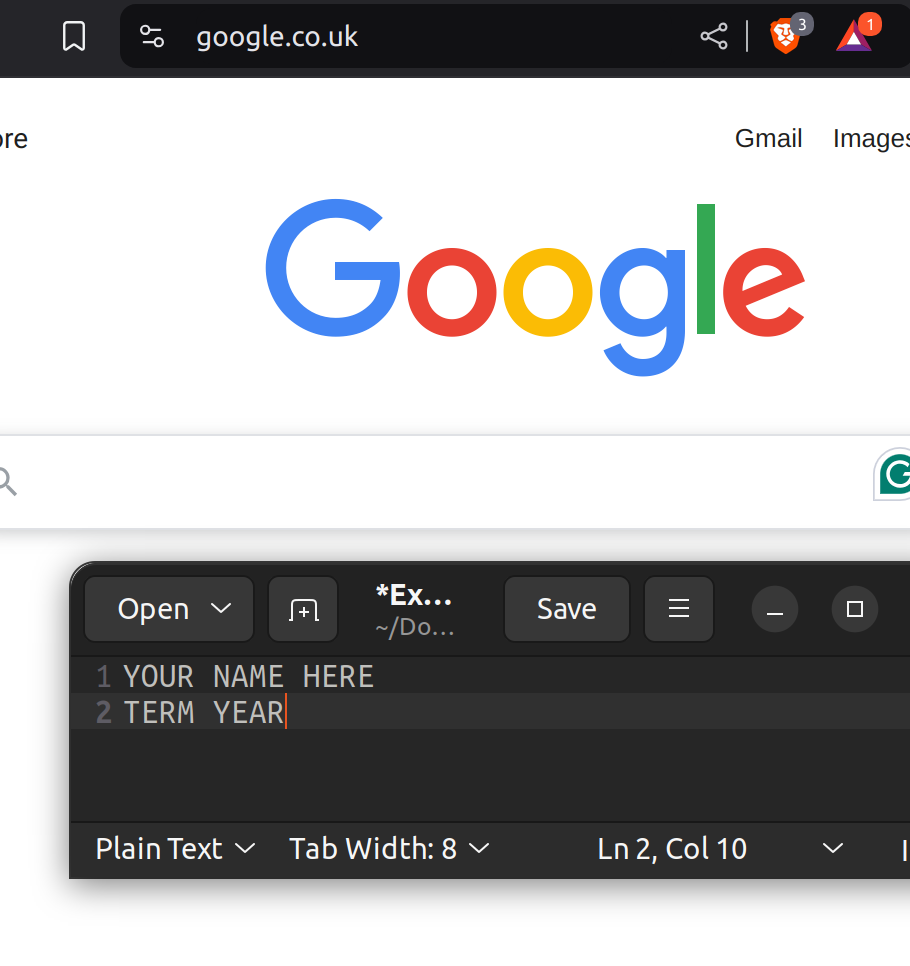
\includegraphics[scale=.2]{ExampleScreenshot.png}}
    \caption{This is an image of what each of your screenshots should look like}

    \end{figure} 


References, a video, a PowerPoint and some notes are available at my website \url {https://www.aholdengouveia.name/IntroData/dataforeveryone.html}

\subsection*{Answer the Following questions about your data}
    \begin{enumerate}
        \item How did you find your data?
        \item Why did you decide on this type of data?
        \item What trends or patterns can be observed?
        \item Are there any outliers or significant data points?
        \item What are at least 3 things you've noticed about your data? 
        \item How did you decide on your column naming?
        \item What was the biggest challenge you had while collecting your data?
        \item Can you see any obvious mistakes or issues with your data? If yes, what are they?
        \item What do you think would be the best way to present this data to others? 
        \item What, if anything, have you learned from collecting this data?
        \item If you had to collect this data again, what might you change?
    \end{enumerate}





\section*{Deliverables:}
This lab should have 2 files submitted, the raw data file and a document with everything else clearly labelled. 
\begin{enumerate}
    \item Raw Data as either a CSV or spreadsheet
    \item Answers to the listed questions
    \item At least 1 visualization of your data, as a whole or parts depending on what you think is best.  Make sure to explain why you chose what you did. 
    \item Screenshot of your visualization that you created
    \item Screenshot of a visualization created by an AI of your choice, make sure to list which AI you used and why you picked that one.
    \item Screenshot of your data
\end{enumerate}

\end{document}